% Strata Cobot - course presentation.
% Built on Overleaf's "An example of the beamer package" (Learn LaTeX: Beamer):
% the Madrid theme, a title page with short title, subtitle, authors with \inst and a
% date, and an outline at the start of every section.
% Compiles with pdfLaTeX (Overleaf default) or XeLaTeX.
\documentclass{beamer}
\usetheme{Madrid}
\usepackage{graphicx}
\usepackage{booktabs}
\usepackage{array}
\newcolumntype{L}[1]{>{\raggedright\arraybackslash}p{#1}}
\usepackage{amsmath}
\graphicspath{{figures/}}

% Ore colours, used consistently with the figures.
\definecolor{azurite}{HTML}{3D8FE6}
\definecolor{malachite}{HTML}{2F9E44}
\definecolor{vanadinite}{HTML}{E8590C}

%Information to be included in the title page:
\title[Strata Cobot] %optional
{Strata Cobot}

\subtitle{Autonomous ore sorting and haulage with two robots in ROS~2}

\author[Reddy, Chowdary, Reddy] % (optional, for multiple authors)
{C~Saihardhik~Reddy \and R~Gagan~Chowdary \and K~Charan~Saatvikh~Reddy}

\institute[Amrita] % (optional)
{
  Robotics course project\\
  Amrita Vishwa Vidyapeetham
}

\date[2026] % (optional)
{October 2026}

% An outline at the start of every section, as in the template.
\AtBeginSection[]
{
  \begin{frame}
    \frametitle{Outline}
    \tableofcontents[currentsection]
  \end{frame}
}

\begin{document}

\frame{\titlepage}

% ======================================================================
\section{Introduction}

\begin{frame}
\frametitle{Two robots, one mining mission}
\begin{columns}[T]
\column{0.52\textwidth}
\begin{enumerate}
  \item \textbf{eBot crosses the site} \\ plans its own route around the rocks
  \item \textbf{eBot takes on the ore} \\ collects an ore package at the drop pose
  \item \textbf{Arm sees each ore} \\ RGB-D camera finds every ore in 3D
  \item \textbf{Arm sorts it} \\ magnet picks each ore and drops it in its container
\end{enumerate}
\column{0.46\textwidth}
\begin{block}{Three minerals, three containers}
  \textcolor{azurite}{\rule{8pt}{8pt}}~Azurite (blue)\\[3pt]
  \textcolor{malachite}{\rule{8pt}{8pt}}~Malachite (green)\\[3pt]
  \textcolor{vanadinite}{\rule{8pt}{8pt}}~Vanadinite (orange)
\end{block}
\begin{alertblock}{Our constraint}
  No MoveIt~2, no Nav2: every planner and controller written from scratch.
\end{alertblock}
\end{columns}
\end{frame}

\begin{frame}
\frametitle{Four goals, each with a number to check}
\centering
\small
\begin{tabular}{@{}L{0.2\textwidth}L{0.14\textwidth}L{0.36\textwidth}L{0.22\textwidth}@{}}
\toprule
\textbf{Subsystem} & \textbf{Robot} & \textbf{Goal} & \textbf{Measured by} \\
\midrule
Perception & Arm camera & Locate every ore in 3D and name its mineral & error vs.\ ground truth \\
Manipulation & UR7e arm & Pick each ore, drop it in its container & ores sorted correctly \\
Path planning & eBot & Collision-free path for each leg & length vs.\ shortest \\
Path following & eBot & Track each path, stop on each pose & tracking error \\
\bottomrule
\end{tabular}
\end{frame}

\begin{frame}
\frametitle{Four nodes, two sense--plan--act pipelines}
\centering
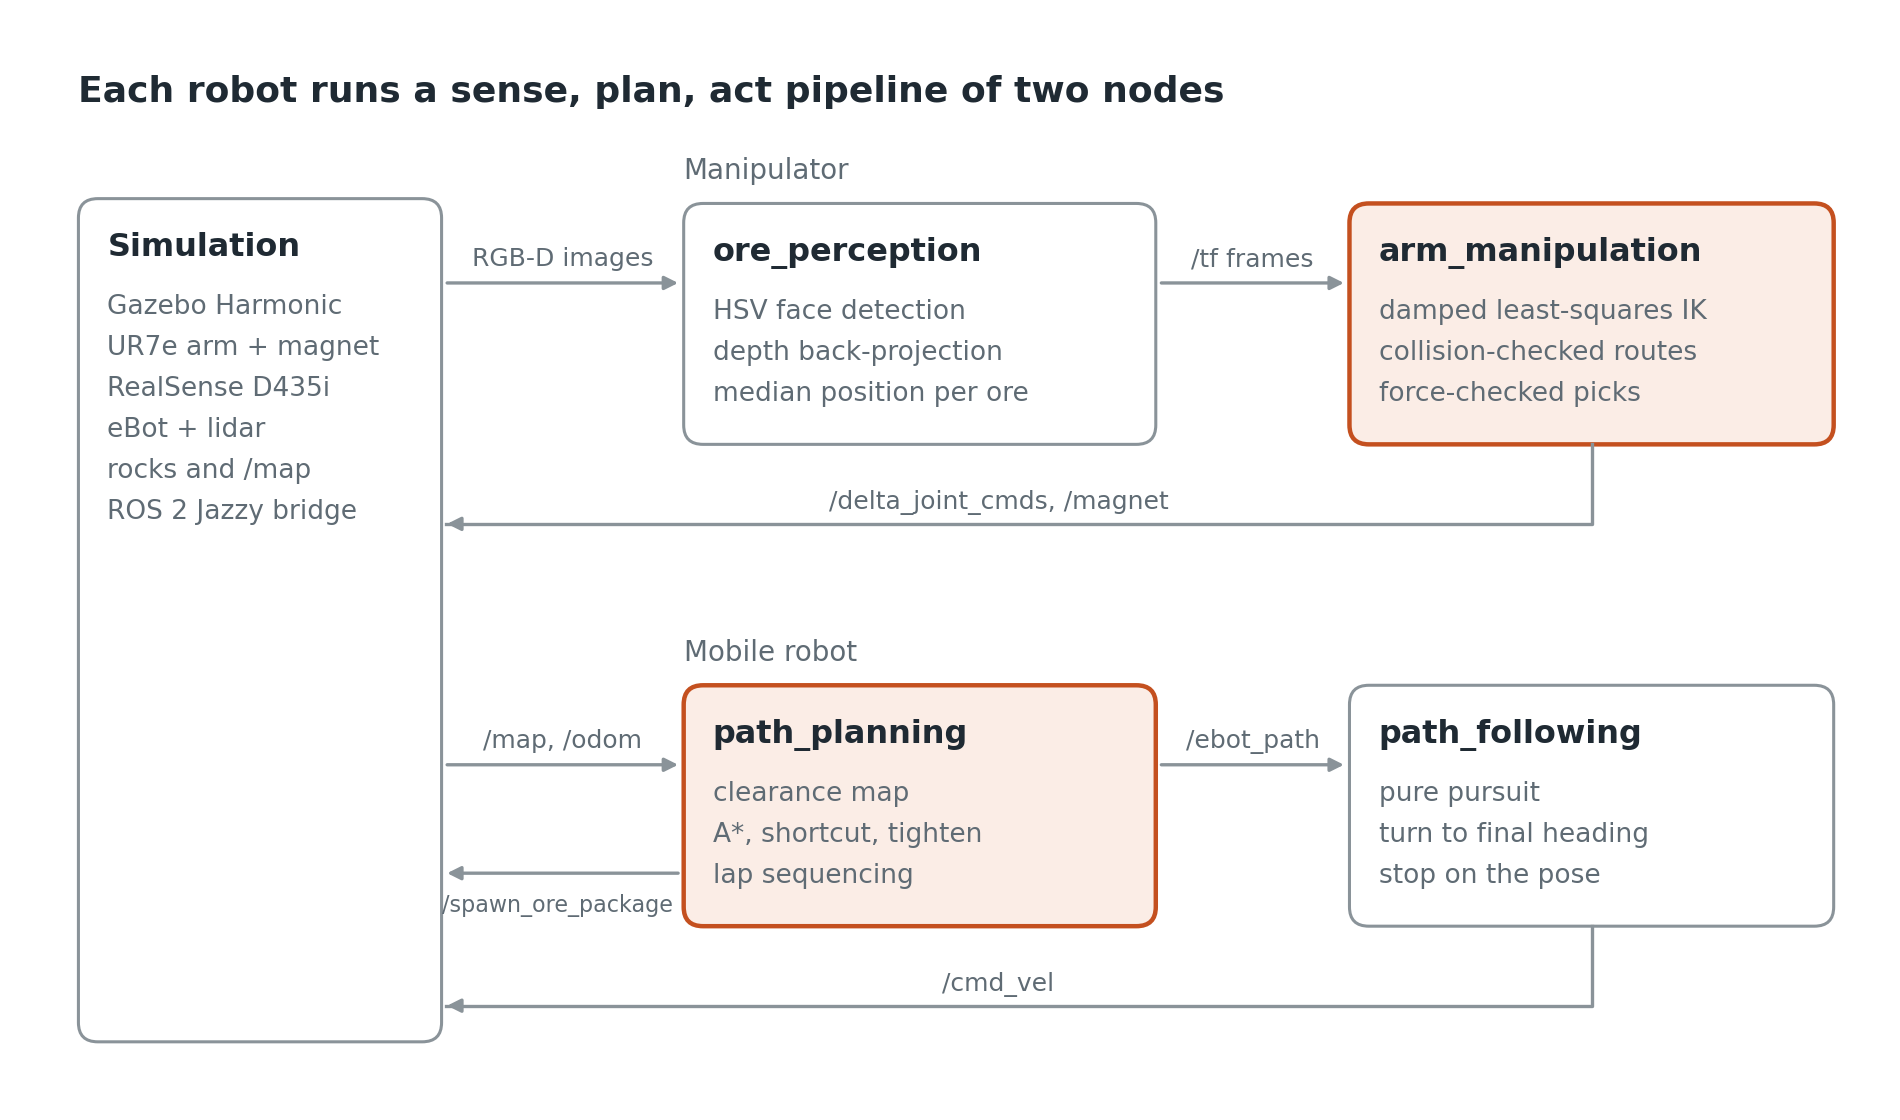
\includegraphics[width=0.9\textwidth]{architecture.png}\\[2pt]
\footnotesize The arm accepts only joint velocities and the eBot only velocity twists,
so every node closes its own control loop at 20--50~Hz.
\end{frame}

% ======================================================================
\section{The manipulator}

\begin{frame}
\frametitle{Find each ore by shape, name it by a colour vote}
\begin{columns}[T]
\column{0.5\textwidth}
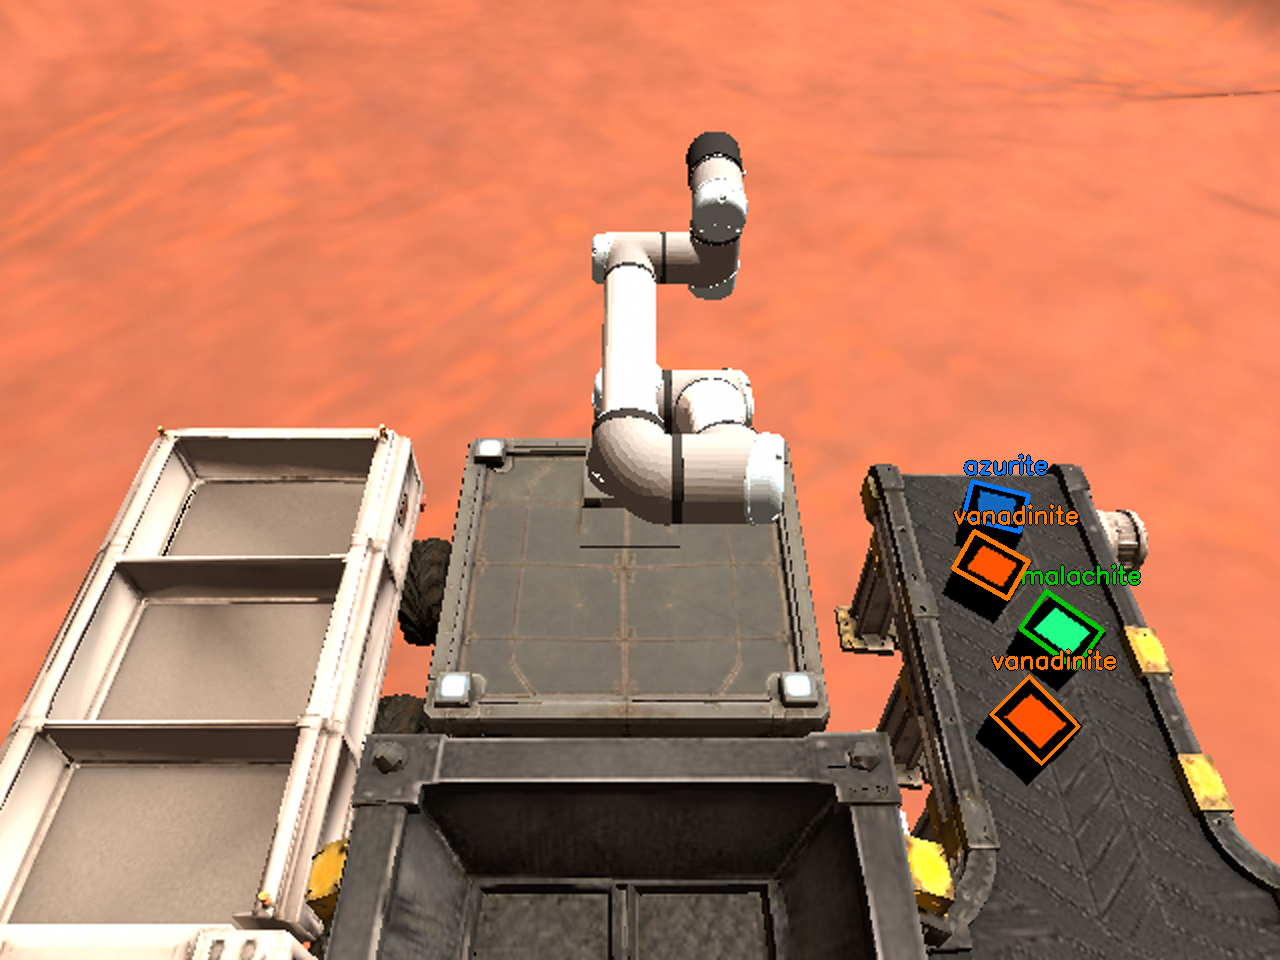
\includegraphics[width=\textwidth]{detection.png}
\column{0.48\textwidth}
\begin{block}{Where: depth}
  An ore's top face is the only surface 66--86~mm above the belt.
  Centre of a rectangle fitted to it: \textbf{2--3~mm} error.
\end{block}
\begin{block}{What: colour vote}
  Share of the face in each mineral's colour (HSV hue).
  The winner needs $\geq$3\% and $2\times$ the runner-up, else \emph{uncertain}.
  Majority vote over 20 frames.
\end{block}
\end{columns}
\end{frame}

\begin{frame}
\frametitle{Real ores are rarely one colour, so we vote}
\begin{columns}[T]
\column{0.56\textwidth}
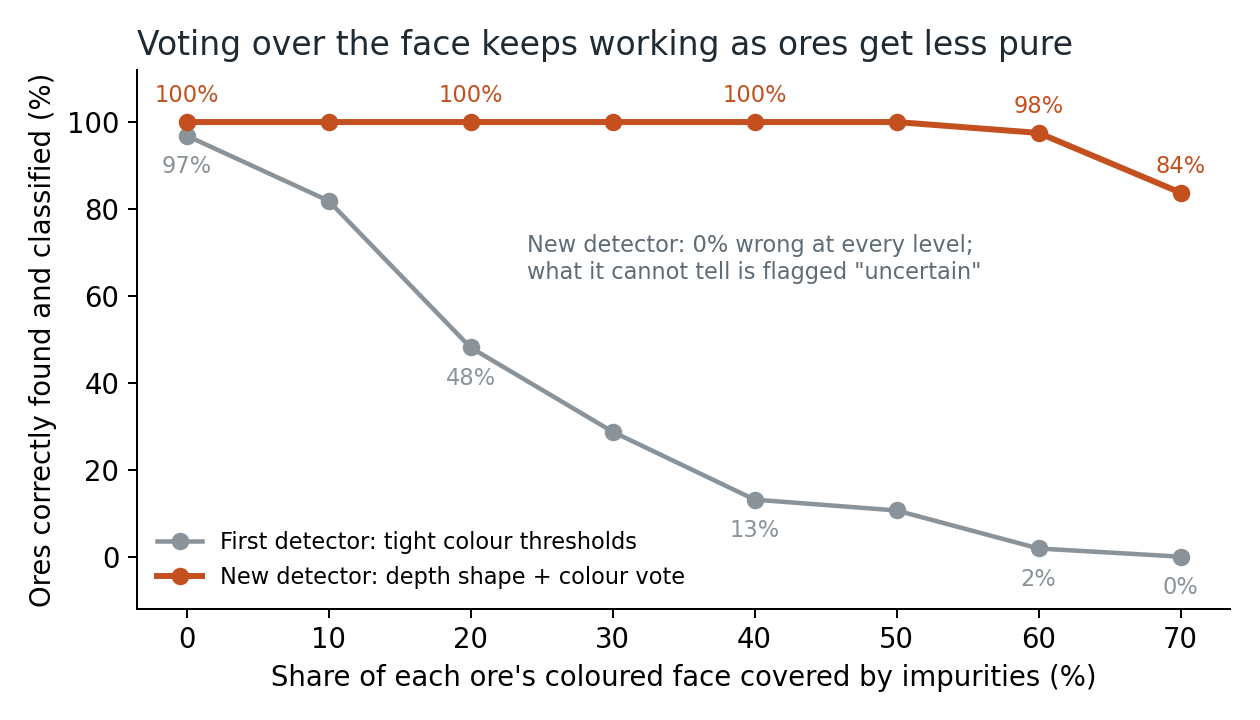
\includegraphics[width=\textwidth]{impurity_robustness.png}\\
\scriptsize Impurities painted into a real camera frame, varied lighting; 160 ores per level.
\column{0.42\textwidth}
\small 180 real museum photos (Wikimedia Commons); calibrated on 90, tested on 90 others:\\[4pt]
\begin{tabular}{@{}lcc@{}}
\toprule
\textbf{Held-out} & \textbf{Tight} & \textbf{Vote} \\
\midrule
Azurite & 10\% & 37\% \\
Malachite & 7\% & 80\% \\
Vanadinite & 17\% & 93\% \\
\midrule
\textbf{All} & \textbf{11\%} & \alert{\textbf{70\%}} \\
\bottomrule
\end{tabular}\\[4pt]
\scriptsize Azurite is hardest: very dark, often crusted with green malachite.
\end{columns}
\end{frame}

\begin{frame}
\frametitle{The containers were found by measuring the rover mesh}
\begin{columns}[T]
\column{0.48\textwidth}
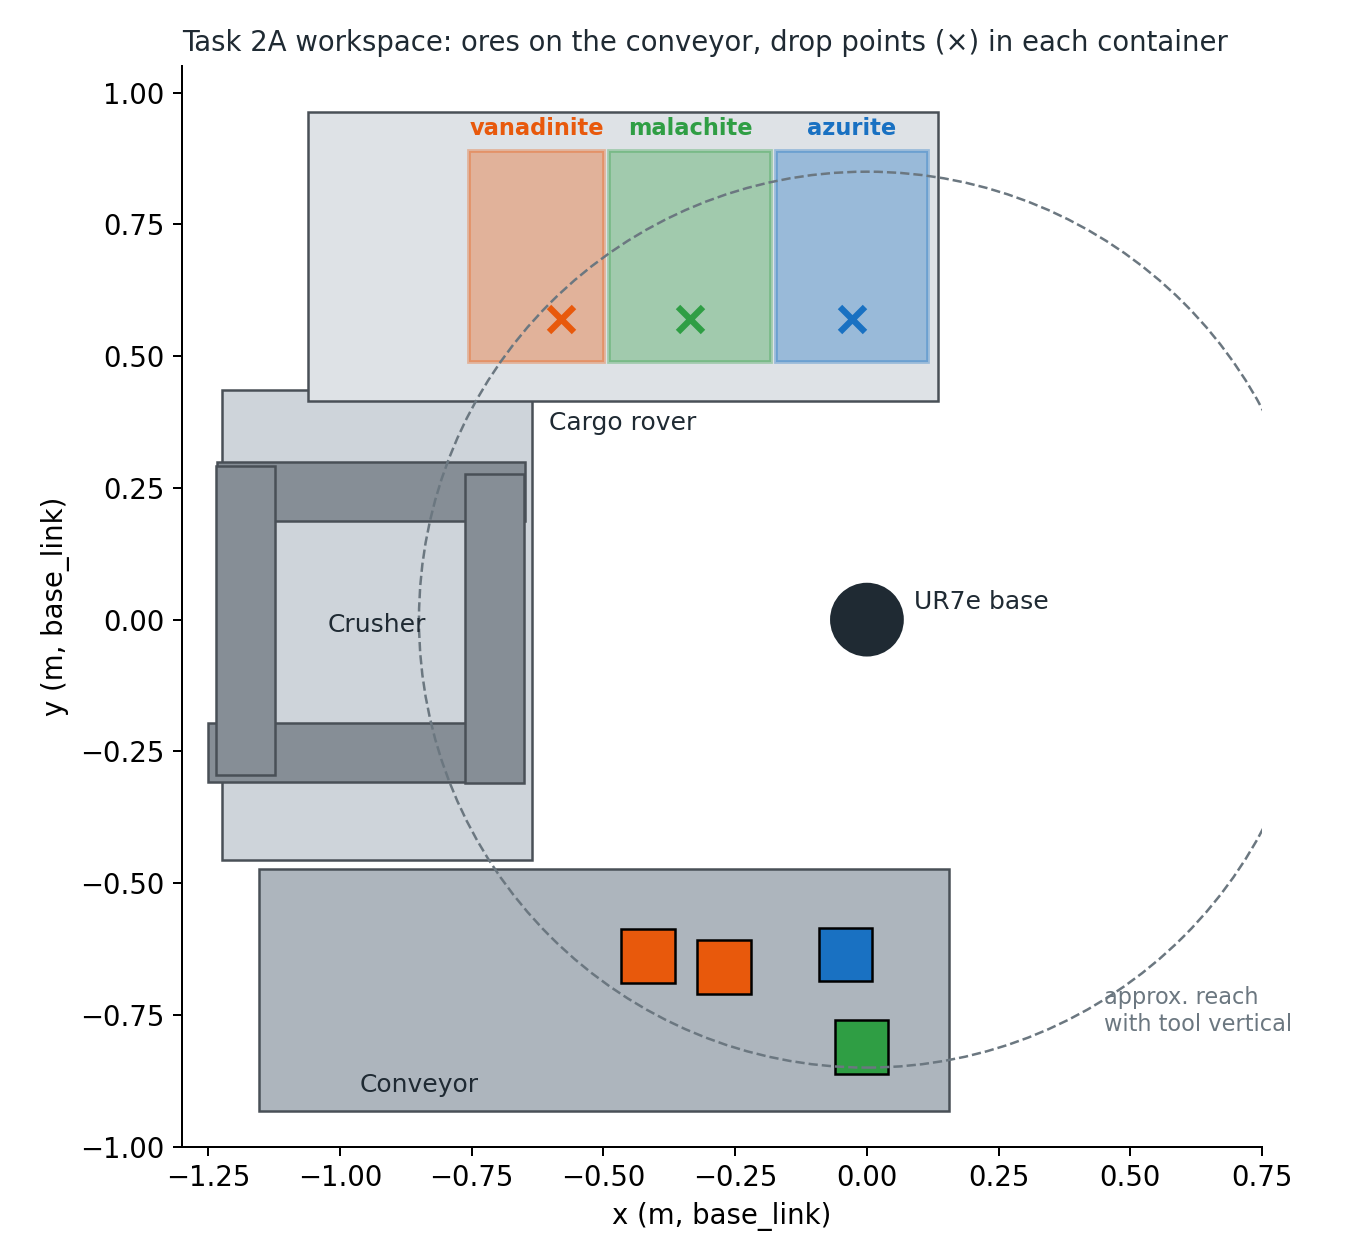
\includegraphics[width=\textwidth]{workspace.png}
\column{0.5\textwidth}
\begin{itemize}
  \item Not given: parsed the cargo rover's collision mesh (GLB) into \texttt{base\_link}
  \item Gazebo's default view: vanadinite nearest, malachite middle, azurite farthest
  \item Vanadinite centre is \textbf{0.93~m} away: out of reach with the tool vertical
  \item So each ore is released at the nearest reachable point inside its container
\end{itemize}
\end{columns}
\end{frame}

\begin{frame}
\frametitle{Every pick is confirmed by the force sensor}
\begin{enumerate}
  \item \textbf{Hover} 10~cm above the face, tool vertical
  \item \textbf{Align} the last millimetres on \texttt{/tcp\_pose\_raw}; magnet on
  \item \textbf{Descend} at 4 then 1.2~cm/s; stop at the face or at 2.5~N
  \item \textbf{Lift and check}: 1.47~N means one 0.15~kg ore is held; under 0.8~N, retry
  \item \textbf{Drop}: carry with the ore in the collision model, release
\end{enumerate}
\vspace{6pt}
\begin{columns}[T]
\column{0.32\textwidth}\centering {\Large\textbf{81~mm}}\\ \footnotesize magnet disc on a 101.6~mm face
\column{0.32\textwidth}\centering {\Large\textbf{1.47~N}}\\ \footnotesize one ore held
\column{0.32\textwidth}\centering {\Large\textbf{0}}\\ \footnotesize safety stops in all trials
\end{columns}
\end{frame}

\begin{frame}
\frametitle{A purpose-built IK solver plans 300$\times$ faster}
\begin{block}{Damped least squares, 5 constraints (position + vertical tool axis)}
\[
\Delta q = J^{T}\left(J J^{T} + \lambda^{2} I\right)^{-1} e, \qquad \lambda = 0.02
\]
\end{block}
\begin{itemize}
  \item Rotation about the vertical is free: the magnet face is round
  \item Safety checked once on the result: joint limits, 3~cm clearance, singularity ($\sigma_{\min} \geq 0.04$), tilt $\leq 1^\circ$
  \item Every solved pose is reused as a seed, so the arm always finds its way back
  \item Straight vertical moves by resolved-rate control: $\dot q = J^{+}[v;\,\omega]$
\end{itemize}
\vspace{4pt}
\centering SLSQP optimiser: \textbf{minutes} per plan \quad$\longrightarrow$\quad DLS: \alert{\textbf{0.1--0.4~s}}
\end{frame}

% ======================================================================
\section{The mobile robot}

\begin{frame}
\frametitle{A*, then shortcut, then tighten}
\begin{columns}[T]
\column{0.58\textwidth}
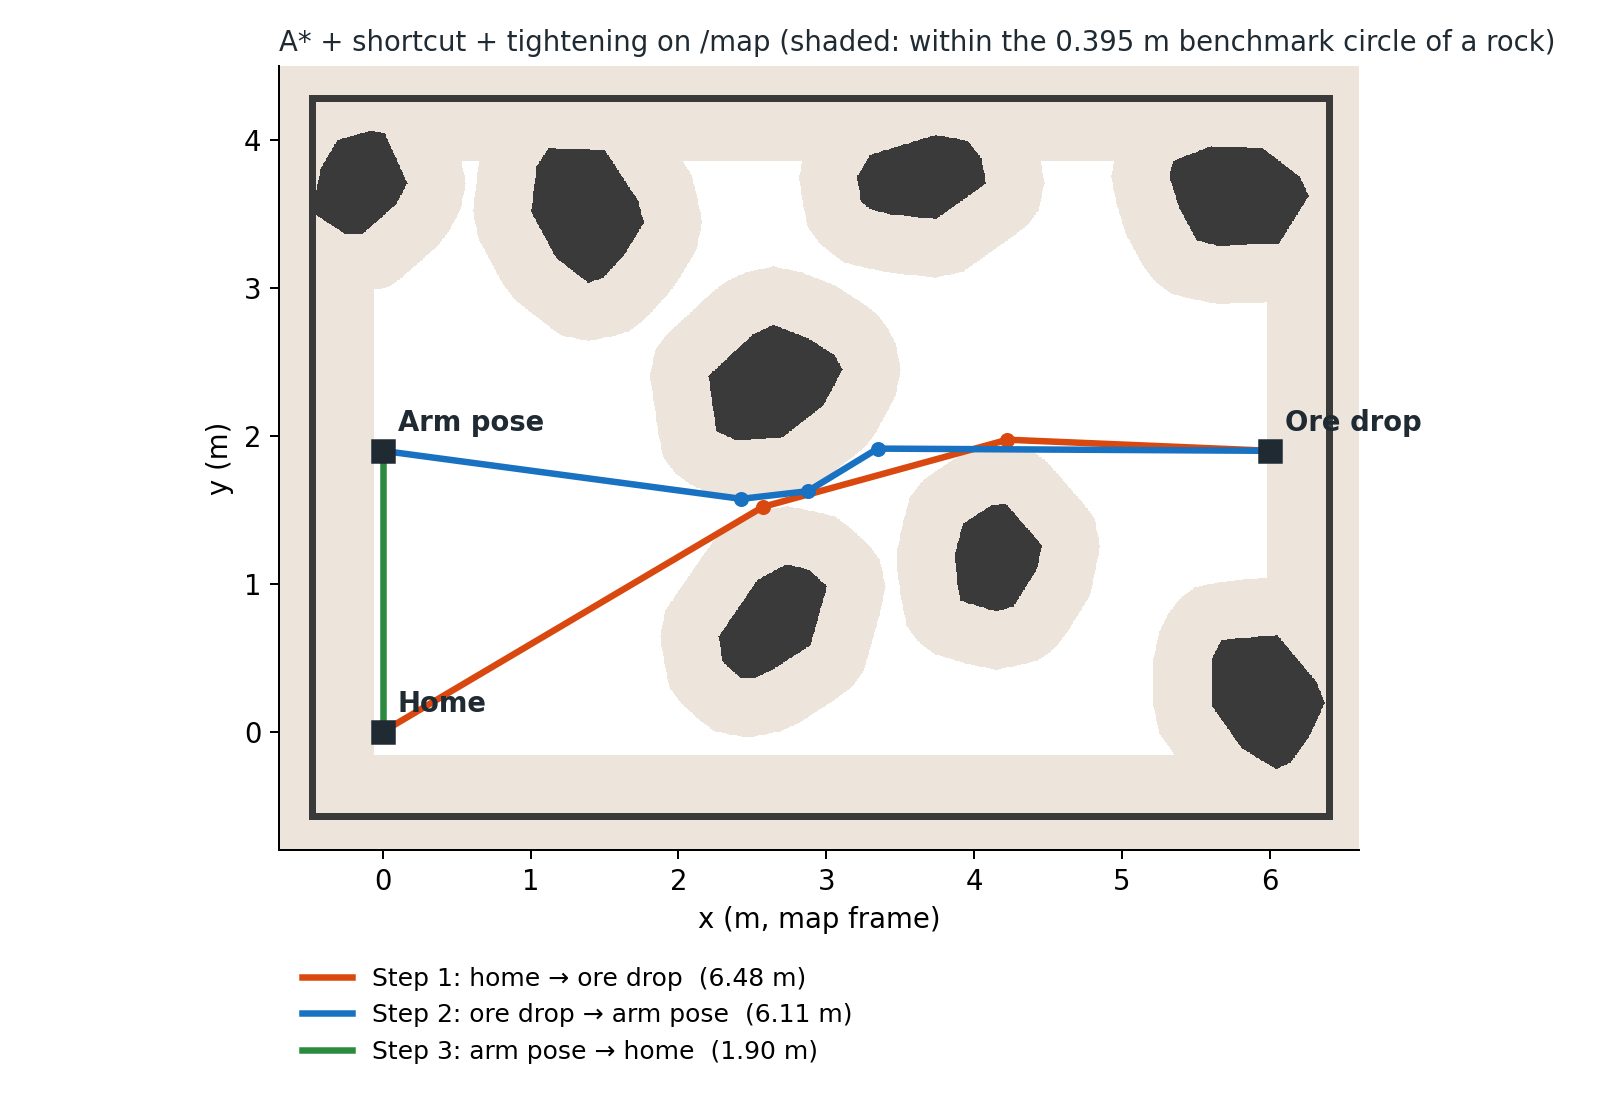
\includegraphics[width=\textwidth]{paths.png}
\column{0.4\textwidth}
\begin{enumerate}
  \item \textbf{Clearance map}: distance transform of the 5~mm \texttt{/map}
  \item \textbf{A*}: 8-connected, 5~cm grid, only cells with enough clearance
  \item \textbf{Shortcut}: jump to the furthest visible point
  \item \textbf{Tighten}: pull each corner in until the legs just clear
\end{enumerate}
\end{columns}
\end{frame}

\begin{frame}
\frametitle{Below 0.40~m clearance, paths stop getting shorter}
\begin{columns}[T]
\column{0.56\textwidth}
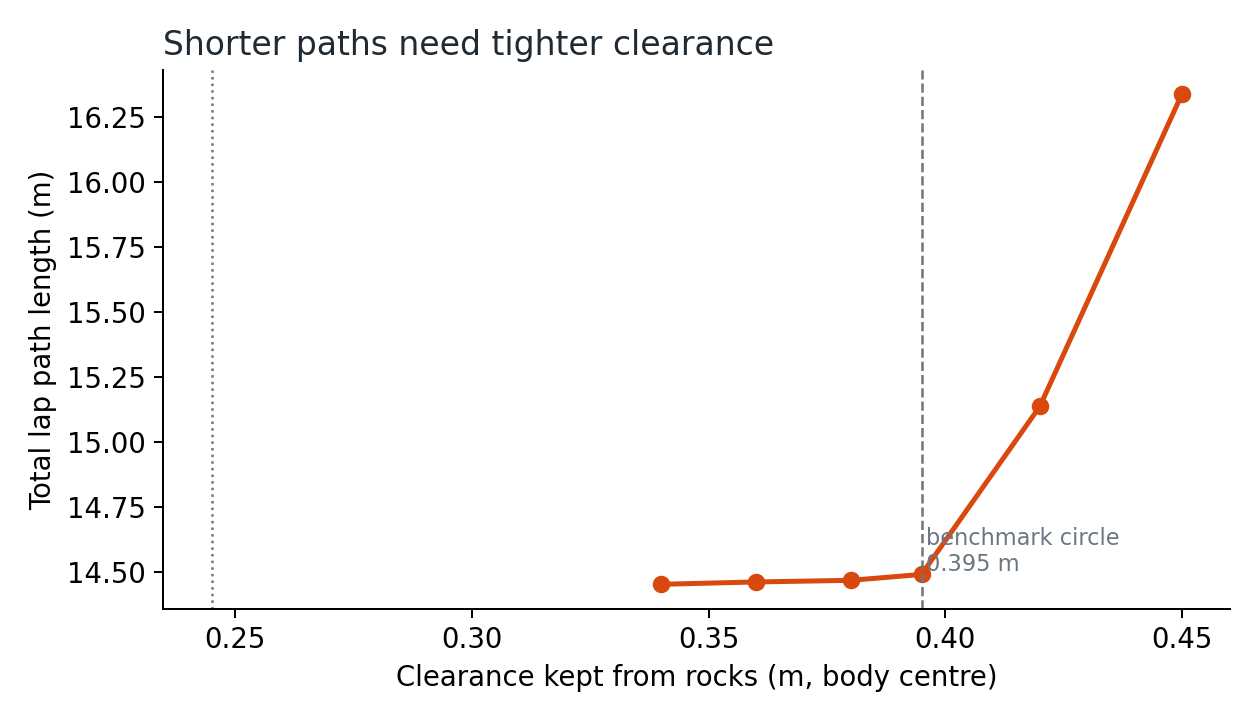
\includegraphics[width=\textwidth]{tradeoff.png}
\column{0.42\textwidth}
\begin{itemize}
  \item Reference path: the robot as a \textbf{0.395~m} circle
  \item Driving straight, only the \textbf{0.245~m} half-width faces a rock
  \item We take the safest clearance (0.40--0.34~m) no longer than the reference
  \item At 0.38~m: 13.5~cm each side; tracking error $\leq$ 9~cm
\end{itemize}
\end{columns}
\end{frame}

\begin{frame}
\frametitle{Pure pursuit follows each path}
\begin{itemize}
  \item Steer to a point 0.30~m ahead on the path
  \item Turn rate $\omega = \mathrm{clip}(2.2\, e_\theta, \pm 1)$; speed $v = 0.35 \cos^2 e_\theta$
  \item Above 40$^\circ$ of heading error: turn on the spot first
  \item At the end: turn to the path's final heading and stop
  \item The lidar only slows the robot; the path is already clear of every rock
\end{itemize}
\end{frame}

% ======================================================================
\section{Results}

\begin{frame}
\frametitle{Every ore sorted, every lap completed, no collisions}
\begin{columns}[T]
\column{0.3\textwidth}
\centering
{\Huge\textbf{16/16}}\\ \footnotesize ores sorted correctly, 4 trials\\[10pt]
{\Huge\textbf{1.00}}\\ \footnotesize best path efficiency
\column{0.68\textwidth}
\small
\begin{tabular}{@{}lL{0.72\linewidth}@{}}
\toprule
\textbf{Trial} & \textbf{Outcome} \\
\midrule
Arm 1--2 & 4/4 sorted each; one ore 0.83~m away \\
Arm 3--4 & New colour-vote perception: 4/4 each \\
Robot 1 & First planner: 14.74~m vs 14.46~m reference \\
Robot 2 & Final planner: 14.55~m vs 14.58~m ($\eta = 1.00$) \\
Robot 3 & Final planner: 14.48~m vs 14.43~m \\
\bottomrule
\end{tabular}\\[4pt]
\footnotesize No collision and no safety stop in any trial; tracking within 0.09~m.
\end{columns}
\end{frame}

\begin{frame}
\frametitle{Live dashboard: one click runs a mission}
\begin{columns}[T]
\column{0.49\textwidth}
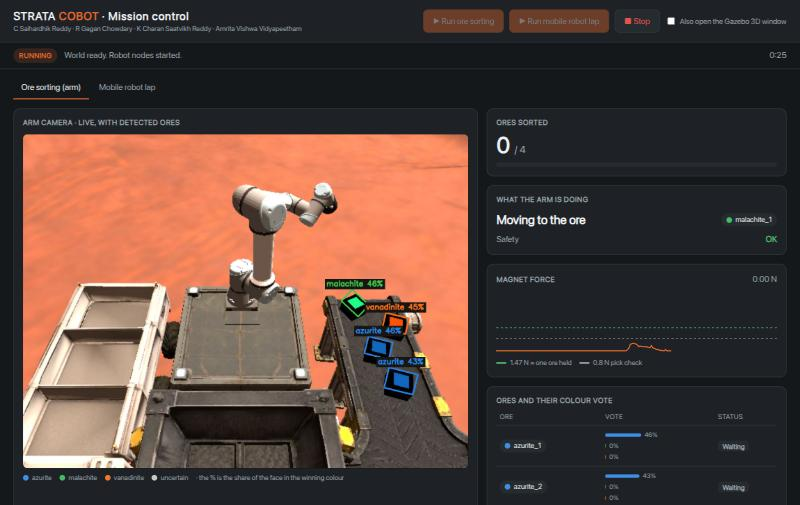
\includegraphics[width=\textwidth]{dashboard_sorting.jpg}\\
\footnotesize Ore sorting: camera with ore labels, arm step, magnet force, votes
\column{0.49\textwidth}
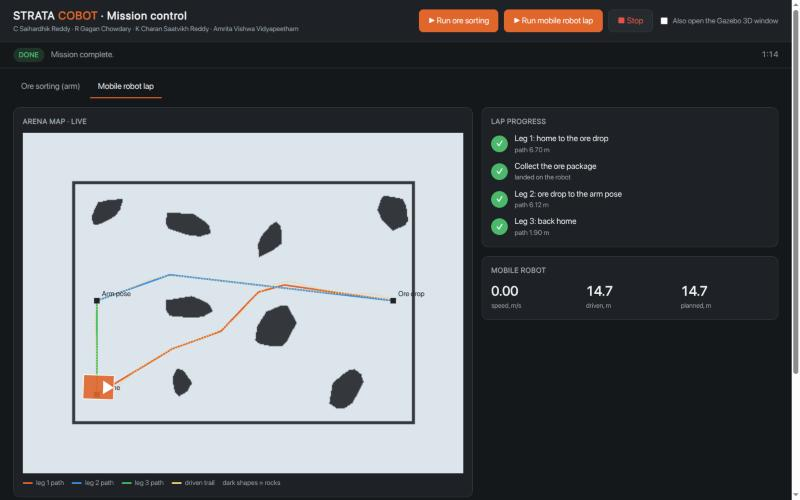
\includegraphics[width=\textwidth]{dashboard_lap.jpg}\\
\footnotesize Mobile robot lap: map, planned legs, robot to scale, progress
\end{columns}
\end{frame}

\begin{frame}
\frametitle{Re-planning around a rock the map does not have}
\begin{columns}[T]
\column{0.55\textwidth}
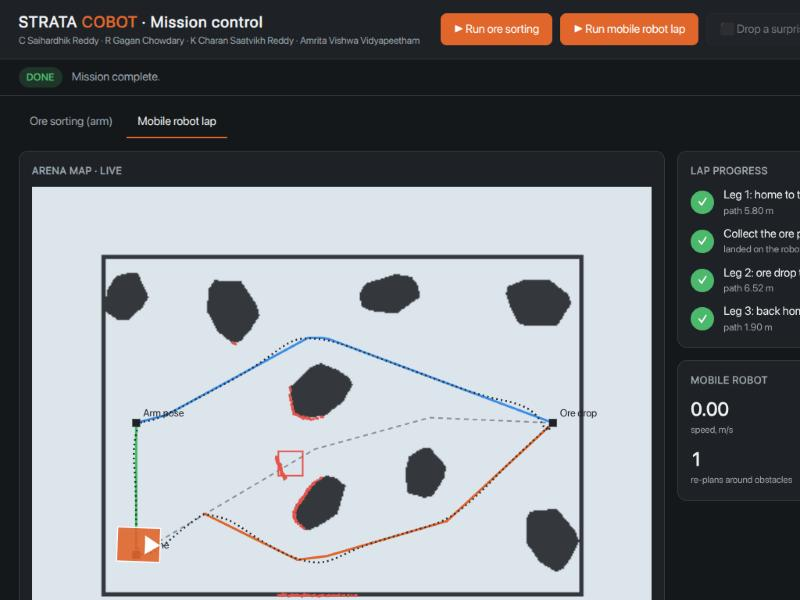
\includegraphics[width=\textwidth]{dashboard_replan.jpg}
\column{0.43\textwidth}
\begin{itemize}
  \item Planned paths keep $\geq$0.30~m from every mapped rock
  \item So a lidar return within 0.26~m of the path ahead is \textbf{new}: the eBot stops
  \item The planner adds it to the map and re-plans from where the eBot stands \alert{in 0.1~s}
  \item Demo: a surprise rock dropped mid-leg; lap completed, never closer than 1.16~m
\end{itemize}
\end{columns}
\end{frame}

\begin{frame}
\frametitle{The full mission: haul, hand off, return}
\begin{columns}[T]
\column{0.55\textwidth}
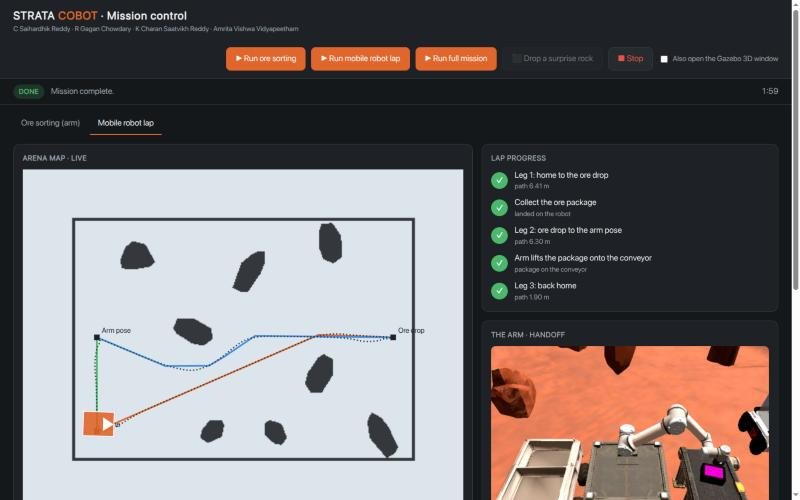
\includegraphics[width=\textwidth]{dashboard_mission.jpg}
\column{0.43\textwidth}
\begin{enumerate}
  \item eBot collects the ore package and drives to the arm
  \item Arm finds it (odometry + depth, \textbf{4~mm}), picks it: \textbf{2.94~N} = 0.30~kg held
  \item Lifts it clear of the deck, sets it on the conveyor intake
  \item eBot drives home
\end{enumerate}
\vspace{4pt}
\footnotesize One click on the dashboard; about 2 minutes end to end.
\end{columns}
\end{frame}

\begin{frame}
\frametitle{What broke, and how we fixed it}
\small
\begin{tabular}{@{}L{0.27\textwidth}L{0.66\textwidth}@{}}
\toprule
\textbf{Problem} & \textbf{Cause and fix} \\
\midrule
No path at all & Drop pose 0.375~m from a wall; full-resolution clearance fixed it \\
Paths 2\% too long & Grid-snapped corners; tightening reached efficiency 1.00 \\
IK took minutes & Checks inside every optimiser step; DLS with one final check \\
Arm lost after a drop & No IK seed back; a library of solved poses \\
Vanadinite unreachable & Release at the nearest reachable point \\
Impure ores & Shape from depth + colour vote, tested on real photos \\
\bottomrule
\end{tabular}
\end{frame}

% ======================================================================
\section{Conclusion}

\begin{frame}
\frametitle{Both robots complete their missions end to end}
\begin{columns}[T]
\column{0.5\textwidth}
\begin{block}{Done}
\begin{itemize}
  \item Sorting: 16/16 ores in the right container
  \item Planning: paths as short as the reference
  \item Robust to impure ores: 70\% on real photos
  \item Hand-off: eBot to arm to conveyor
  \item Re-planning around unmapped rocks
\end{itemize}
\end{block}
\column{0.46\textwidth}
\begin{exampleblock}{Next}
\begin{itemize}
  \item Train a classifier on real ore samples
  \item Move to physical robots
\end{itemize}
\end{exampleblock}
\end{columns}
\vspace{10pt}
\centering \Large Thank you \quad$\cdot$\quad Questions?
\end{frame}

\end{document}
